\documentclass[12pt, a4paper]{article}

\usepackage[margin=1.8cm,top=2cm,bottom=2cm]{geometry}
\usepackage{amsmath,amssymb,amsfonts}
\usepackage{graphicx}
\usepackage[colorlinks=true,linkcolor=blue,citecolor=blue,urlcolor=blue]{hyperref}
\usepackage{bm,xcolor}
\usepackage[numbers,sort&compress]{natbib}
\usepackage{titlesec}
\usepackage{float}

\newcommand{\Geff}{G_{\mathrm{eff}}}
\newcommand{\cs}{c_s}
\newcommand{\meff}{m_{\mathrm{eff}}}
\newcommand{\heff}{\hbar_{\mathrm{eff}}}
\newcommand{\rhob}{\bar{\rho}}
\newcommand{\vb}{\bar{v}}
\newcommand{\Phieff}{\Phi_{\mathrm{eff}}}
\newcommand{\lP}{\ell_{\mathrm{P}}}
\newcommand{\mP}{m_{\mathrm{P}}}

\begin{document}

\title{Emergent Newtonian Gravity from the Collective Acoustic Metric\\of a Logarithmic Superfluid Vacuum}

\author{B.~B.~Kulangiev\\\small{Haifa, Israel}}
\date{April 2026}
\maketitle

\begin{abstract}
\noindent In a companion paper, we showed that the Painlev\'{e}-Gullstrand (PG) flow $v = \sqrt{2GM/r}$ regularizes the static-metric pathology of the logarithmic superfluid vacuum, yielding the PPN parameter $\gamma = 1$ for any barotropic equation of state. Here we derive this macroscopic flow as a collective mean-field effect of $N$ microscopic vortex-Gausson solitons---the topological defects of the logarithmic condensate. We show that the self-consistency requirement selects the PG flow uniquely: the static solution fails catastrophically (the spatial-to-temporal metric ratio diverges at the background equation-of-state exponent $\alpha = -1$), while the PG flow closes the self-consistency loop exactly. Postulating that each soliton sources the acoustic metric through a localized perturbation, we derive the emergent gravitational constant $\Geff \sim c^2/(\xi^2\rho_0)$, where $\xi$ is the healing length and $\rho_0$ is the vacuum condensate mass density. This expression is universal---independent of the source mass $M$ and the distance $r$. Matching $\Geff$ to Newton's constant, combined with the natural condensate packing density $n_0 \sim 1/\xi^3$, determines $\xi \sim \ell_P$ (the Planck length) and $\rho_0 \sim m_P/\ell_P^3$ (the Planck density). An independent derivation from the Bernoulli relation of the logarithmic fluid confirms that Newtonian gravity ($\delta\rho \propto 1/r$) requires exactly the PG velocity profile ($v^2 \propto 1/r$). The continuity constraint is discussed as an open problem.
\end{abstract}


% ====================================================================
\section{Introduction}
\label{sec:intro}
% ====================================================================

In a companion paper~\cite{kulangiev_2026}, we established that a superfluid vacuum model based on the relativistic logarithmic Klein-Gordon equation, analyzed via the Madelung decomposition, provides the structural ingredients needed to recover general relativistic light bending ($\gamma = 1$). The key results were:

(i) The kinematic trap: any real scalar field gives $\gamma = 0$, regardless of the self-interaction potential~\cite{will_2014}.

(ii) The Madelung escape: the complex field's hydrodynamic representation introduces a density-dependent sound speed and a macroscopic flow velocity.

(iii) The static pathology: the static acoustic metric gives $\gamma_{\mathrm{static}} = (1-\alpha)/(1+\alpha)$, which has a pole at $\alpha = -1$. The relativistic logarithmic equation of state at the background density gives precisely $\alpha = -1$, making the static acoustic metric mathematically ill-defined.

(iv) The PG solution: the flowing acoustic metric with $v(r) = \sqrt{2\Geff M/r}$ gives $\gamma = 1$ exactly, and is the unique self-consistent weak-field configuration.

The central open problem identified in~\cite{kulangiev_2026} was the derivation of the macroscopic PG flow from the microscopic soliton dynamics. In this paper, we close this gap. We show that the collective effect of $N$ vortex-Gausson solitons embedded in the logarithmic condensate produces a macroscopic gravitational potential $\Phi = -\Geff M/r$ through the coarse-grained acoustic metric, and that the self-consistency of this metric uniquely selects the PG flow. We derive the emergent gravitational constant $\Geff$ in terms of microscopic parameters and show that matching it to Newton's $G$ determines the vacuum condensate density.


% ====================================================================
\section{Framework: The Coarse-Grained Condensate}
\label{sec:framework}
% ====================================================================

\subsection{Microscopic and macroscopic scales}

The vacuum condensate is described by a complex order parameter $\psi(x,t)$ satisfying the relativistic logarithmic Klein-Gordon equation~\cite{rosen_1969,bartkowski_gorka_2008}, the relativistic counterpart of the logarithmic Schr\"{o}dinger equation~\cite{bialynicki_birula_1979}:
\begin{equation}
    \Box\psi + \mu^2\psi - b\,\psi\,\ln\!\left(\frac{|\psi|^2}{\rho_0}\right) = 0\,,
\label{eq:log_kg}
\end{equation}
with healing length $\xi = \heff/(\meff \cs)$ setting the microscopic scale. The Madelung decomposition $\psi = \sqrt{\rho}\,e^{iS/\heff}$ yields a continuity equation and a Hamilton-Jacobi equation coupling the condensate density $\rho$ and flow velocity $\mathbf{v} = \nabla S/\meff$~\cite{kulangiev_2026}.

\paragraph{Two distinct densities}
A dimensional clarification: in the relativistic Lagrangian $\mathcal{L} = \rho X - V(\rho)$ with $X = \partial_\mu S\,\partial^\mu S$, the variable $\rho = |\psi|^2$ has units of inverse-energy-volume, not mass density~\cite{kulangiev_2026}. The physical mass density of the condensate, the quantity one would measure as kg/m$^3$, is computed from the time-time component of the stress-energy tensor:
\begin{equation}
    \rho_{\mathrm{mass}} = T_{00}/c^2 = [\rho V'(\rho) + V(\rho)]/c^2\,,
\label{eq:rho_mass_def}
\end{equation}
which at the background reduces to a constant. Throughout this paper, when $\rho_0$ appears in dimensional formulae for the gravitational coupling (Eqs.~\ref{eq:G_eff}, \ref{eq:planck_scale}), we mean $\rho_0^{\mathrm{phys}} = T_{00}/c^2$ at the background; when $\rho$ or $\rho_0$ appears in the field equations and Bernoulli relations (Eqs.~\ref{eq:log_kg}, \ref{eq:bernoulli_log}), we mean the Lagrangian variable. The two are linearly related at fixed background through Eq.~(\ref{eq:rho_mass_def}); the conversion factor is absorbed into the O(1) prefactors of the dimensional analysis below.

In the superfluid vacuum model, fundamental particles are topological defects---vortex-Gaussons---with core size $\sim\xi$ and energy $E_v$~\cite{bialynicki_birula_1979,avdeenkov_2011}. A macroscopic gravitating body (star, planet) consists of $N = M/m$ such solitons, where $M$ is the total mass and $m$ is the mass per particle. The gravitational field is measured at distances $r \gg R_{\mathrm{star}} \gg N^{1/3}\xi$, far from any individual soliton.

We introduce a coarse-graining scale $\ell$ satisfying $\xi \ll \ell \ll r$ and define:
\begin{align}
    \rhob(r) &= \langle|\psi|^2\rangle_\ell\,,
    & &\text{(macroscopic condensate density)}\\
    \vb(r) &= \langle\mathbf{v}\rangle_\ell\,,
    & &\text{(macroscopic flow velocity)}\\
    \rho_{\mathrm{mass}}(r) &= n(r)\cdot m\,,
    & &\text{(particle mass density)}
\end{align}
where $n(r)$ is the number density of solitons. The macroscopic condensate density $\rhob$ is conceptually distinct from the particle mass density $\rho_{\mathrm{mass}}$: the former describes the vacuum substrate, the latter describes the matter embedded within it.

\newpage
\subsection{Coarse-grained equations}

After coarse-graining, the condensate obeys the steady-state Euler equations:
\begin{align}
    \nabla\cdot(\rhob\,\vb) &= -\mathcal{S}(r)\,,
\label{eq:cg_continuity}\\
    \tfrac{1}{2}\vb^2 + h(\rhob) + \Phieff &= \text{const}\,,
\label{eq:cg_bernoulli}
\end{align}
where $\mathcal{S}(r) = n(r)\cdot\Gamma_{\mathrm{sink}}$ is the sink rate from soliton core absorption, $h(\rhob) = \int c_s^2(\rhob)\,d\rhob/\rhob$ is the specific enthalpy, and $\Phieff$ is the gravitational potential defined by the acoustic metric. For the logarithmic equation of state~\cite{barcelo_2005,kulangiev_2026} with $c_s^2 = c^2 / [2\ln(\rhob/\rho_c)+3]$:
\begin{equation}
    h(\rhob) = \tfrac{1}{2}\,\ln\!\left[2\ln(\rhob/\rho_c) + 3\right]\,c^2\,.
\end{equation}


% ====================================================================
\section{The Self-Consistency Argument}
\label{sec:self_consistency}
% ====================================================================

In the superfluid vacuum framework, the gravitational potential is not an externally specified quantity. It \emph{is} the acoustic metric: phonons (including photons) propagate on the effective geometry defined by the condensate's density $\rhob$ and flow velocity $\vb$, and what observers interpret as gravity is the response of these excitations to the condensate's spatial structure. Physical spacetime remains flat; the apparent ``curvature'' is an emergent property of how perturbations propagate through the underlying fluid. This imposes a self-consistency requirement.

\subsection{The acoustic metric potential}

The acoustic metric in Painlev\'{e}-Gullstrand form is~\cite{unruh_1981,visser_1998}:
\begin{equation}
    ds^2 = \frac{\rhob}{\cs}\!\left[-(c_s^2 - \vb^2)\,dt^2 - 2\vb\,dr\,dt + dr^2 + r^2 d\Omega^2\right]\,.
\label{eq:acoustic_metric}
\end{equation}
Transforming to Schwarzschild-like coordinates via $dT = dt + \vb\,dr/(c_s^2 - \vb^2)$:
\begin{align}
    g_{TT} &= -\frac{\rhob}{\cs}(c_s^2 - \vb^2)\,,\\
    g_{rr} &= \frac{\rhob\,\cs}{c_s^2 - \vb^2}\,.
\end{align}
The effective Newtonian potential is read off from the temporal component:
\begin{equation}
    \Phieff = -\frac{1}{2}\frac{\delta g_{TT}}{g_{TT}}\bigg|_{\text{far field}}\,.
\label{eq:phi_from_metric}
\end{equation}

\subsection{Solution A: Static (\texorpdfstring{$\vb = 0$}{v=0})}

With no flow, the density perturbation $\epsilon = \delta\rhob/\rho_0$ creates~\cite{kulangiev_2026}:
\begin{equation}
    \frac{\delta g_{TT}}{g_{TT}} = (1+\alpha)\,\epsilon\,,\qquad
    \frac{\delta g_{rr}}{g_{rr}} = (1-\alpha)\,\epsilon\,,
\end{equation}
where $\alpha = d\ln c_s / d\ln\rho$. The corresponding PPN parameter is
\begin{equation}
    \gamma_{\mathrm{static}} = \frac{1-\alpha}{1+\alpha}\,.
\label{eq:gamma_static}
\end{equation}
For the relativistic logarithmic equation of state at the background density, $\alpha = -1$~\cite{kulangiev_2026}, and the denominator of~(\ref{eq:gamma_static}) vanishes:
\begin{equation}
    \gamma_{\mathrm{static}} \to \infty\quad\text{at}\quad \alpha = -1\,.
\label{eq:gamma_pathology}
\end{equation}
The static acoustic metric is mathematically pathological: the spatial metric perturbation diverges relative to the temporal one, and no finite weak-field expansion around the static background exists. Physically, the pole signals that the static configuration is not a stable background for perturbations of the density alone. Any consistent treatment must therefore introduce additional dynamical content beyond the static density channel; this is the role of the macroscopic flow developed in Sec.~\ref{sec:self_consistency} below.


\subsection{Solution B: Painlev\'{e}-Gullstrand flow \texorpdfstring{($\vb = \sqrt{2\Phieff}$, $\rhob \approx \rho_0$)}{(v = sqrt(2*Phi\_eff), rho approx rho\_0)}}

With $\vb^2 = 2|\Phieff|$ and $\rhob = \rho_0$:
\begin{align}
    g_{TT} &\approx -\rho_0 c_s\,(1 - 2U)\,,\\
    g_{rr} &\approx \frac{\rho_0}{c_s}\,(1 + 2U)\,,
\end{align}
where $U = \Geff M/(c_s^2 r)$ is the dimensionless potential. This gives $\Phieff = -\Geff M/r$ and $\gamma = 1$.

The Bernoulli equation verifies self-consistency: with $\vb^2 = 2|\Phieff|$ and $\Phieff = -\Geff M/r < 0$, we have $\tfrac{1}{2}\vb^2 + \Phieff = |\Phieff| - |\Phieff| = 0$, which is satisfied identically. The PG flow closes the self-consistency loop for \emph{any} barotropic equation of state, because the Painlev\'{e}-Gullstrand acoustic metric is identically the Schwarzschild metric in rain coordinates~\cite{visser_1998,volovik_2003}.


\subsection{Density correction and its decoupling at \texorpdfstring{$\alpha=-1$}{alpha=-1}}
\label{sec:density_decoupling}

The PG flow does perturb the condensate density. The fluid's own Bernoulli relation---the linearized Hamilton-Jacobi equation with \emph{no} externally inserted potential (Sec.~\ref{sec:bernoulli})---reads $\tfrac{1}{2}\vb^2 + \tilde{c}_s^2\,\epsilon = 0$, giving a genuine first-order depletion
\begin{equation}
    \epsilon \equiv \frac{\delta\rhob}{\rho_0} = -\frac{\vb^2}{2\tilde{c}_s^2} = -2U \neq 0\,,
\label{eq:epsilon_depletion}
\end{equation}
where $\tilde{c}_s^2 = \heff^2 b_R/(2\meff^2) = c^2/2$ is the stiffness of the Hamilton-Jacobi flow-density relation, fixed exactly by the Gausson invariant $b_R\sigma^2=1$ with $\sigma=\xi$~\cite{kulangiev_2026e}, and $U = \Geff M/(c^2 r) > 0$. The density does not vanish around a gravitating mass; it is depleted at $O(U)$.

What vanishes is the \emph{gravitational effect} of this depletion. Expanding the temporal metric component $g_{TT} = -(\rhob/c_s)(c_s^2 - \vb^2)$ to first order with $c_s \propto \rhob^{\,\alpha}$ separates a density channel from a flow channel:
\begin{equation}
    \frac{\delta g_{TT}}{g_{TT}^{(0)}} = (1+\alpha)\,\epsilon \;-\; \frac{\vb^2}{c_s^2}\,.
\label{eq:gtt_two_channel}
\end{equation}
At the background density the logarithmic equation of state gives $\alpha = -1$, so the density coefficient $(1+\alpha)$ vanishes identically and the depletion drops out of $g_{TT}$ regardless of its magnitude. After Minkowski normalization the temporal component is sourced by the flow alone,
\begin{equation}
    \Phieff\big|_{\alpha=-1} = -\tfrac{1}{2}\vb^2\,,
\label{eq:phi_eff_flow}
\end{equation}
so the Newtonian potential, light bending, and clock rates carry no first-order trace of $\epsilon$. This is the temporal-component counterpart of the static pole (Eq.~\ref{eq:gamma_pathology}): at $\alpha = -1$ the density channel cannot carry the metric, so the flow must. The $O(U)$ depletion is real but gravitationally invisible to first order; second-order corrections are $O(U^2) \sim 10^{-12}$ at the solar limb, negligible for all solar system tests.


% ====================================================================
\section{Independent Confirmation from Bernoulli Dynamics}
\label{sec:bernoulli}
% ====================================================================

The Hamilton-Jacobi equation of the logarithmic fluid fixes the velocity profile---but through the flow, not through a density well. We stress that this equation contains \emph{no} externally inserted gravitational potential: in the emergent picture the potential is read off the acoustic metric, not added to the fluid's equation of motion.

\subsection{The genuine Bernoulli depletion}

Linearizing Eq.~(\ref{eq:log_kg}) in the Madelung representation about the background (rest-mass phase $\partial_t S = -\meff c^2$), with the mostly-plus signature fixed by the d'Alembertian and $b > 0$~\cite{kulangiev_2026}:
\begin{equation}
    \ln\!\left(\frac{\rho(r)}{\rho_\infty}\right) = -\frac{\meff^2}{b\heff^2}\,|\mathbf{v}(r)|^2\,.
\label{eq:bernoulli_log}
\end{equation}
The minus sign is forced: $|\mathbf{v}|^2$ enters through the spatial (positive) part of the metric and $b>0$ is the condition for the Gausson solitons to exist, so $\ln(\rho/\rho_\infty)<0$. This is a genuine depletion,
\begin{equation}
    \boxed{\;\frac{\delta\rho}{\rho_\infty} = \frac{\meff^2}{b\heff^2}\,v^2 > 0\,,\qquad \delta\rho \equiv \rho_\infty - \rho\;}
\label{eq:bernoulli_relation}
\end{equation}
agreeing with the metric-derived depletion of Sec.~\ref{sec:density_decoupling}, now with the prefactor fixed exactly: the Gausson invariant $b_R\sigma^2=1$~\cite{kulangiev_2026e} together with the core-radius identification $\sigma=\xi$ gives $\meff^2/(b\heff^2) = 1/(2\tilde{c}_s^2)$ with $\tilde{c}_s^2 = c^2/2$, so $\delta\rho/\rho_\infty = v^2/c^2 = 2U$ with no residual $O(1)$ freedom.

\subsection{Why the density well does not source gravity}

It is tempting to close the argument by Poisson's equation: a Newtonian potential $\Phi \propto 1/r$ would imply a density well $\delta\rho \propto 1/r$, which with Eq.~(\ref{eq:bernoulli_relation}) gives $v^2 \propto 1/r$. This route is \emph{not} valid here. As shown in Sec.~\ref{sec:density_decoupling}, at the background exponent $\alpha = -1$ the density perturbation decouples from the temporal metric: the depletion is real but produces no first-order potential, and there is no ``$\Phi \propto -\delta\rho$'' identification for the Poisson step to act on. The density well comes along for the ride; it does not drive the geometry.

\subsection{The flow-sourced profile}

The potential is carried by the flow. At $\alpha=-1$ the flow-sourced potential is $\Phieff = -\tfrac{1}{2}v^2$ (Eq.~\ref{eq:phi_eff_flow}), and the fluid's equation of motion $\tfrac12 v^2 + \Phieff = 0$ is then satisfied identically---the self-consistency identity that makes PG valid for any barotropic equation of state. The radial profile is fixed by requiring the flow to reproduce the Newtonian potential of a mass $M$, with $\Geff$ derived independently in Sec.~\ref{sec:G_eff}:
\begin{equation}
    \Phieff(r) = -\frac{\Geff M}{r}
    \quad\Longrightarrow\quad
    v(r) = \sqrt{\frac{2\Geff M}{r}}\,.
\label{eq:pg_from_flow}
\end{equation}
Because $\Phieff \propto v^2$, a $1/r$ potential admits only $v^2 \propto 1/r$: the Painlev\'{e}-Gullstrand profile is the unique flow that can carry a Newtonian potential, and the derivation never invokes the density well that the $\alpha=-1$ pole renders gravitationally inert. The alternatives are excluded directly: a rigid circulation $v_\theta \propto 1/r$ gives $\Phieff \propto 1/r^2$ (force $\propto 1/r^3$), and a dipole flow $v \propto 1/r^2$ gives $\Phieff \propto 1/r^4$---both too steep.


% ====================================================================
\section{The Emergent Gravitational Constant}
\label{sec:G_eff}
% ====================================================================

\subsection{The single-soliton ansatz}

We \emph{postulate} that each vortex-Gausson soliton, viewed from distances $r \gg \xi$, sources a localized perturbation of the acoustic metric that produces a Newtonian $1/r$ potential. The dimensional structure of this potential is fixed by the available parameters: the soliton's rest energy $E_v = mc^2$, the condensate mass density $\rho_0$, and the healing length $\xi$. By dimensional analysis, the unique combination with the dimensions of a Newtonian potential and the correct $1/r$ falloff is:
\begin{equation}
    \delta\Phi_{\mathrm{single}}(r) = -\frac{c^2\,m}{4\pi\,\xi^2\,\rho_0\,r}\,,
\label{eq:single_phi}
\end{equation}
up to an O(1) prefactor. We refer to~(\ref{eq:single_phi}) as the \emph{single-soliton ansatz}: a derivation from the linearized coupled Madelung--Hamilton-Jacobi system, which would fix the prefactor explicitly, is left to future work. The qualitative result---a $1/r$ potential sourced by each soliton---follows from the linear-response structure of the condensate; the specific dimensional combination $c^2/(\xi^2\rho_0)$ is the unique form consistent with $[\Phi] = \mathrm{m}^2/\mathrm{s}^2$.

\subsection{Collective potential and emergent G}

For $N = M/m$ identical solitons distributed within a sphere of radius $R_{\mathrm{star}}$, the collective potential at $r \gg R_{\mathrm{star}}$ is:
\begin{equation}
    \Phi_{\mathrm{total}}(r) = N\cdot\delta\Phi_{\mathrm{single}}(r) = -\frac{c^2\,M}{4\pi\,\xi^2\,\rho_0\,r}\,.
\end{equation}
Comparing with the Newtonian potential $\Phi = -\Geff M/r$:
\begin{equation}
    \boxed{\;\Geff \sim \frac{c^2}{\xi^2\,\rho_0}\;}
\label{eq:G_eff}
\end{equation}
where the proportionality absorbs an O(1) prefactor from the detailed Gausson energy integral. Dimensional check: $[c^2/(\xi^2\rho_0)] = (\mathrm{m}^2/\mathrm{s}^2)/(\mathrm{m}^2\cdot\mathrm{kg}/\mathrm{m}^3) = \mathrm{m}^3/(\mathrm{kg\,s}^2) = [G]$ \checkmark.

This expression is \emph{universal}: it depends only on the vacuum condensate parameters ($\rho_0$, $\xi$, $c$), and is independent of the source mass $M$, the distance $r$, and the number of particles $N$.

\subsection{Physical content}

The gravitational constant~(\ref{eq:G_eff}) has a clean physical interpretation: gravity is weak because the vacuum is stiff. The product $\xi^2\rho_0$ has units of mass per length, and combined with $c^2$ controls how strongly a localized energy density perturbs the surrounding condensate. A stiffer condensate (larger $\rho_0$, smaller $\xi$) resists deformation more strongly, producing a smaller potential per unit source mass. Equivalently, the bulk modulus of the vacuum is $K \sim \rho_0\,c^2$, and the gravitational coupling is $\Geff \sim 1/(K\,\xi^2/c^2)$---the inverse of the elastic response per unit healing volume.

\subsection{Determination of the vacuum density and healing length}

Equation~(\ref{eq:G_eff}) contains two unknown vacuum parameters, $\xi$ and $\rho_0$. Matching $\Geff$ to Newton's constant gives one equation:
\begin{equation}
    G \sim \frac{c^2}{\xi^2\,\rho_0}\,.
\label{eq:G_match}
\end{equation}
A second relation is required to fix $\xi$ and $\rho_0$ separately. The natural choice is the condensate packing density $n_0 \sim 1/\xi^3$---one condensate particle per healing volume:
\begin{equation}
    \rho_0 = m_{\mathrm{eff}}\,n_0 \sim \frac{m_{\mathrm{eff}}}{\xi^3}\,,
\label{eq:rho_packing}
\end{equation}
where $m_{\mathrm{eff}}$ is the mass of one condensate particle. Combined with the healing-length relation $\xi = \hbar/(m_{\mathrm{eff}}\,c)$ from the soliton-core balance condition~\cite{kulangiev_2026}, Eqs.~(\ref{eq:G_match})~and~(\ref{eq:rho_packing}) yield:
\begin{equation}
    m_{\mathrm{eff}}^2 \sim \frac{\hbar\,c}{G}\,,\quad\text{i.e.}\quad m_{\mathrm{eff}} \sim m_P\,,
\label{eq:meff_planck}
\end{equation}
where $m_P = \sqrt{\hbar c/G}$ is the Planck mass. The corresponding healing length and density are:
\begin{equation}
    \boxed{\;\xi \sim \lP\,,\qquad \rho_0 \sim \frac{m_P}{\lP^3} \approx 5 \times 10^{96}\;\mathrm{kg/m^3}\,\;}
\label{eq:planck_scale}
\end{equation}
where $\lP = \sqrt{\hbar G/c^3}$ is the Planck length. The vacuum condensate has Planck-mass particles spaced by Planck-length distances, with bulk mass density at the Planck scale. This is the natural maximum density for a relativistic quantum field; the framework therefore predicts a Planck-density vacuum reservoir, with gravitational effects sourced by $O(U \rho_0)$ \emph{perturbations} of this background rather than by the background density itself.

The detailed self-consistency derivation, including O(1) prefactors, is presented separately in the Planck-scale companion paper~\cite{kulangiev_2026e}.


% ====================================================================
\section{Numerical Verification of the Soliton Building Block}
\label{sec:numerics}
% ====================================================================

The derivation of $\Geff$ relies on the existence and stability of vortex-Gausson solitons in the logarithmic condensate. We verify these properties by numerical solution of the two-dimensional logarithmic Gross-Pitaevskii equation:
\begin{equation}
    i\heff\frac{\partial\psi}{\partial t} = -\frac{\heff^2}{2\meff}\nabla^2\psi - b\,\ln\!\left(\frac{|\psi|^2}{\rho_0}\right)\psi\,,
\label{eq:gpe}
\end{equation}
using a split-step Fourier method on a $512^2$ grid with $\heff = \meff = b = \rho_0 = 1$.

\subsection{Ground states}

Imaginary-time evolution with fixed phase topology ($\psi \to |\psi|\,e^{in\theta}$ at each step) yields stationary vortex-Gausson states for winding numbers $n = 0, 1, 2, 3$. The healing length in the simulation's natural units is $\xi = \heff/\sqrt{2\meff b}$ from the soliton-core balance, against which the ground-state widths $\sigma$ are normalized:

\begin{center}
\begin{tabular}{cccccc}
\hline
$n$ & $E$ & $\mu$ & $\sigma/\xi$ & $\rho_{\max}/\rho_0$ & $v_\theta$ scaling \\
\hline
0 & 10.14 & 0.614 & 1.000 & 3.90 & --- \\
1 & 12.60 & 2.363 & 2.054 & 0.43 & $r^{-1.001}$ \\
2 & 11.68 & 3.287 & 3.189 & 0.17 & $r^{-1.001}$ \\
3 & 10.55 & 3.907 & 4.367 & 0.10 & $r^{-1.005}$ \\
\hline
\end{tabular}
\end{center}

The $n = 0$ Gausson width $\sigma = 1.000\,\xi$ matches the exact analytical prediction of Bia\l{}ynicki-Birula and Mycielski~\cite{bialynicki_birula_1979}. The energy is conserved to $\Delta E/|E_0| < 10^{-9}$ during real-time evolution, validating the solver.

\subsection{Topological velocity locking}

The far-field tangential velocity of all vortex states satisfies $v_\theta \propto r^{-1.00}$ to three significant figures. This confirms the topological locking theorem: for any irrotational flow with quantized circulation $\Gamma = n h/\meff$, the velocity is $v_\theta = \Gamma/(2\pi r) \propto 1/r$, regardless of the equation of state. The logarithmic nonlinearity affects only the core structure ($\rho(r)$ near $r = 0$), not the far-field velocity.

This result establishes that a \emph{single} vortex-Gausson cannot produce the PG profile $v \propto r^{-1/2}$. The PG flow must arise as a collective effect of many solitons, as derived in Secs.~\ref{sec:self_consistency}--\ref{sec:G_eff}.

\subsection{PG flow self-consistency and stability}

The preceding subsections verify the soliton building block. We now verify the collective result: that the PG inflow $v = \sqrt{2\Geff M/r}$ with $\rho \approx \rho_0$ is a self-consistent and dynamically stable solution of the coarse-grained Euler equations with the relativistic logarithmic equation of state.

We solve the one-dimensional spherical Euler equations (continuity and momentum) on a radial grid of 4096 points ($r \in [5, 400]$) with the relativistic logarithmic sound speed $c_s^2 = c^2/[2\ln(\rho/\rho_c) + 3]$ (Paper~1~\cite{kulangiev_2026}), a gravitational source $\Phi = -GM/r$, and a distributed sink $\mathcal{S}(r) = \rho_0\,|\nabla\cdot\mathbf{v}_{\mathrm{PG}}|$ balancing the PG flow divergence (Sec.~\ref{sec:continuity}). Time integration uses a third-order TVD Runge-Kutta scheme with CFL number 0.25.

Two cases are evolved for $2 \times 10^5$ time steps ($T \approx 4822$ in units of $r_{\mathrm{min}}/c_s$):

\emph{Case~1:} Exact PG initial conditions ($\rho = \rho_0$, $v = \sqrt{2GM/r}$). The density deviation remains bounded by $|\delta\rho/\rho_0| < 10^{-5}$ and the velocity error stays below $10^{-3}\%$ throughout. The measured velocity power law is $v \propto r^{-0.500}$ to three significant figures. This simulation imposes an external potential $\Phi = -GM/r$ in the momentum equation rather than letting the metric emerge self-consistently; it therefore tests the dynamical stability of the PG configuration, and is consistent with---but does not by itself establish---the gravitational decoupling of the density channel derived in Sec.~\ref{sec:density_decoupling}.

\emph{Case~2:} A 20\% sinusoidal velocity perturbation is imposed on the PG profile. The perturbation decays monotonically with the velocity error decreasing from 12.8\% to 0.02\% over $T \approx 4220$ in units of $r_{\mathrm{min}}/c_s$, and the power law slope recovering to $-0.500$. The final density excursion $|\delta\rho/\rho_0| \approx 4 \times 10^{-5}$ and final velocity error of $0.02\%$ are both consistent with relaxation toward the PG configuration. This demonstrates that the PG flow is not merely a stationary point but a \emph{dynamical attractor}: perturbations are expelled, and the system relaxes to the PG configuration. 

We note that the PG attractor behavior demonstrated here is generic to any barotropic EOS that asymptotes to $c_s \to c$ at the background; the simulation thus verifies the dynamical stability of the PG configuration and the correct functioning of the distributed sink mechanism, but is not a specific test of the relativistic logarithmic equation of state. Tests sensitive to the EOS at higher orders in $\delta\rho/\rho_0$ are deferred to future work.

\begin{figure}[H]
\centering
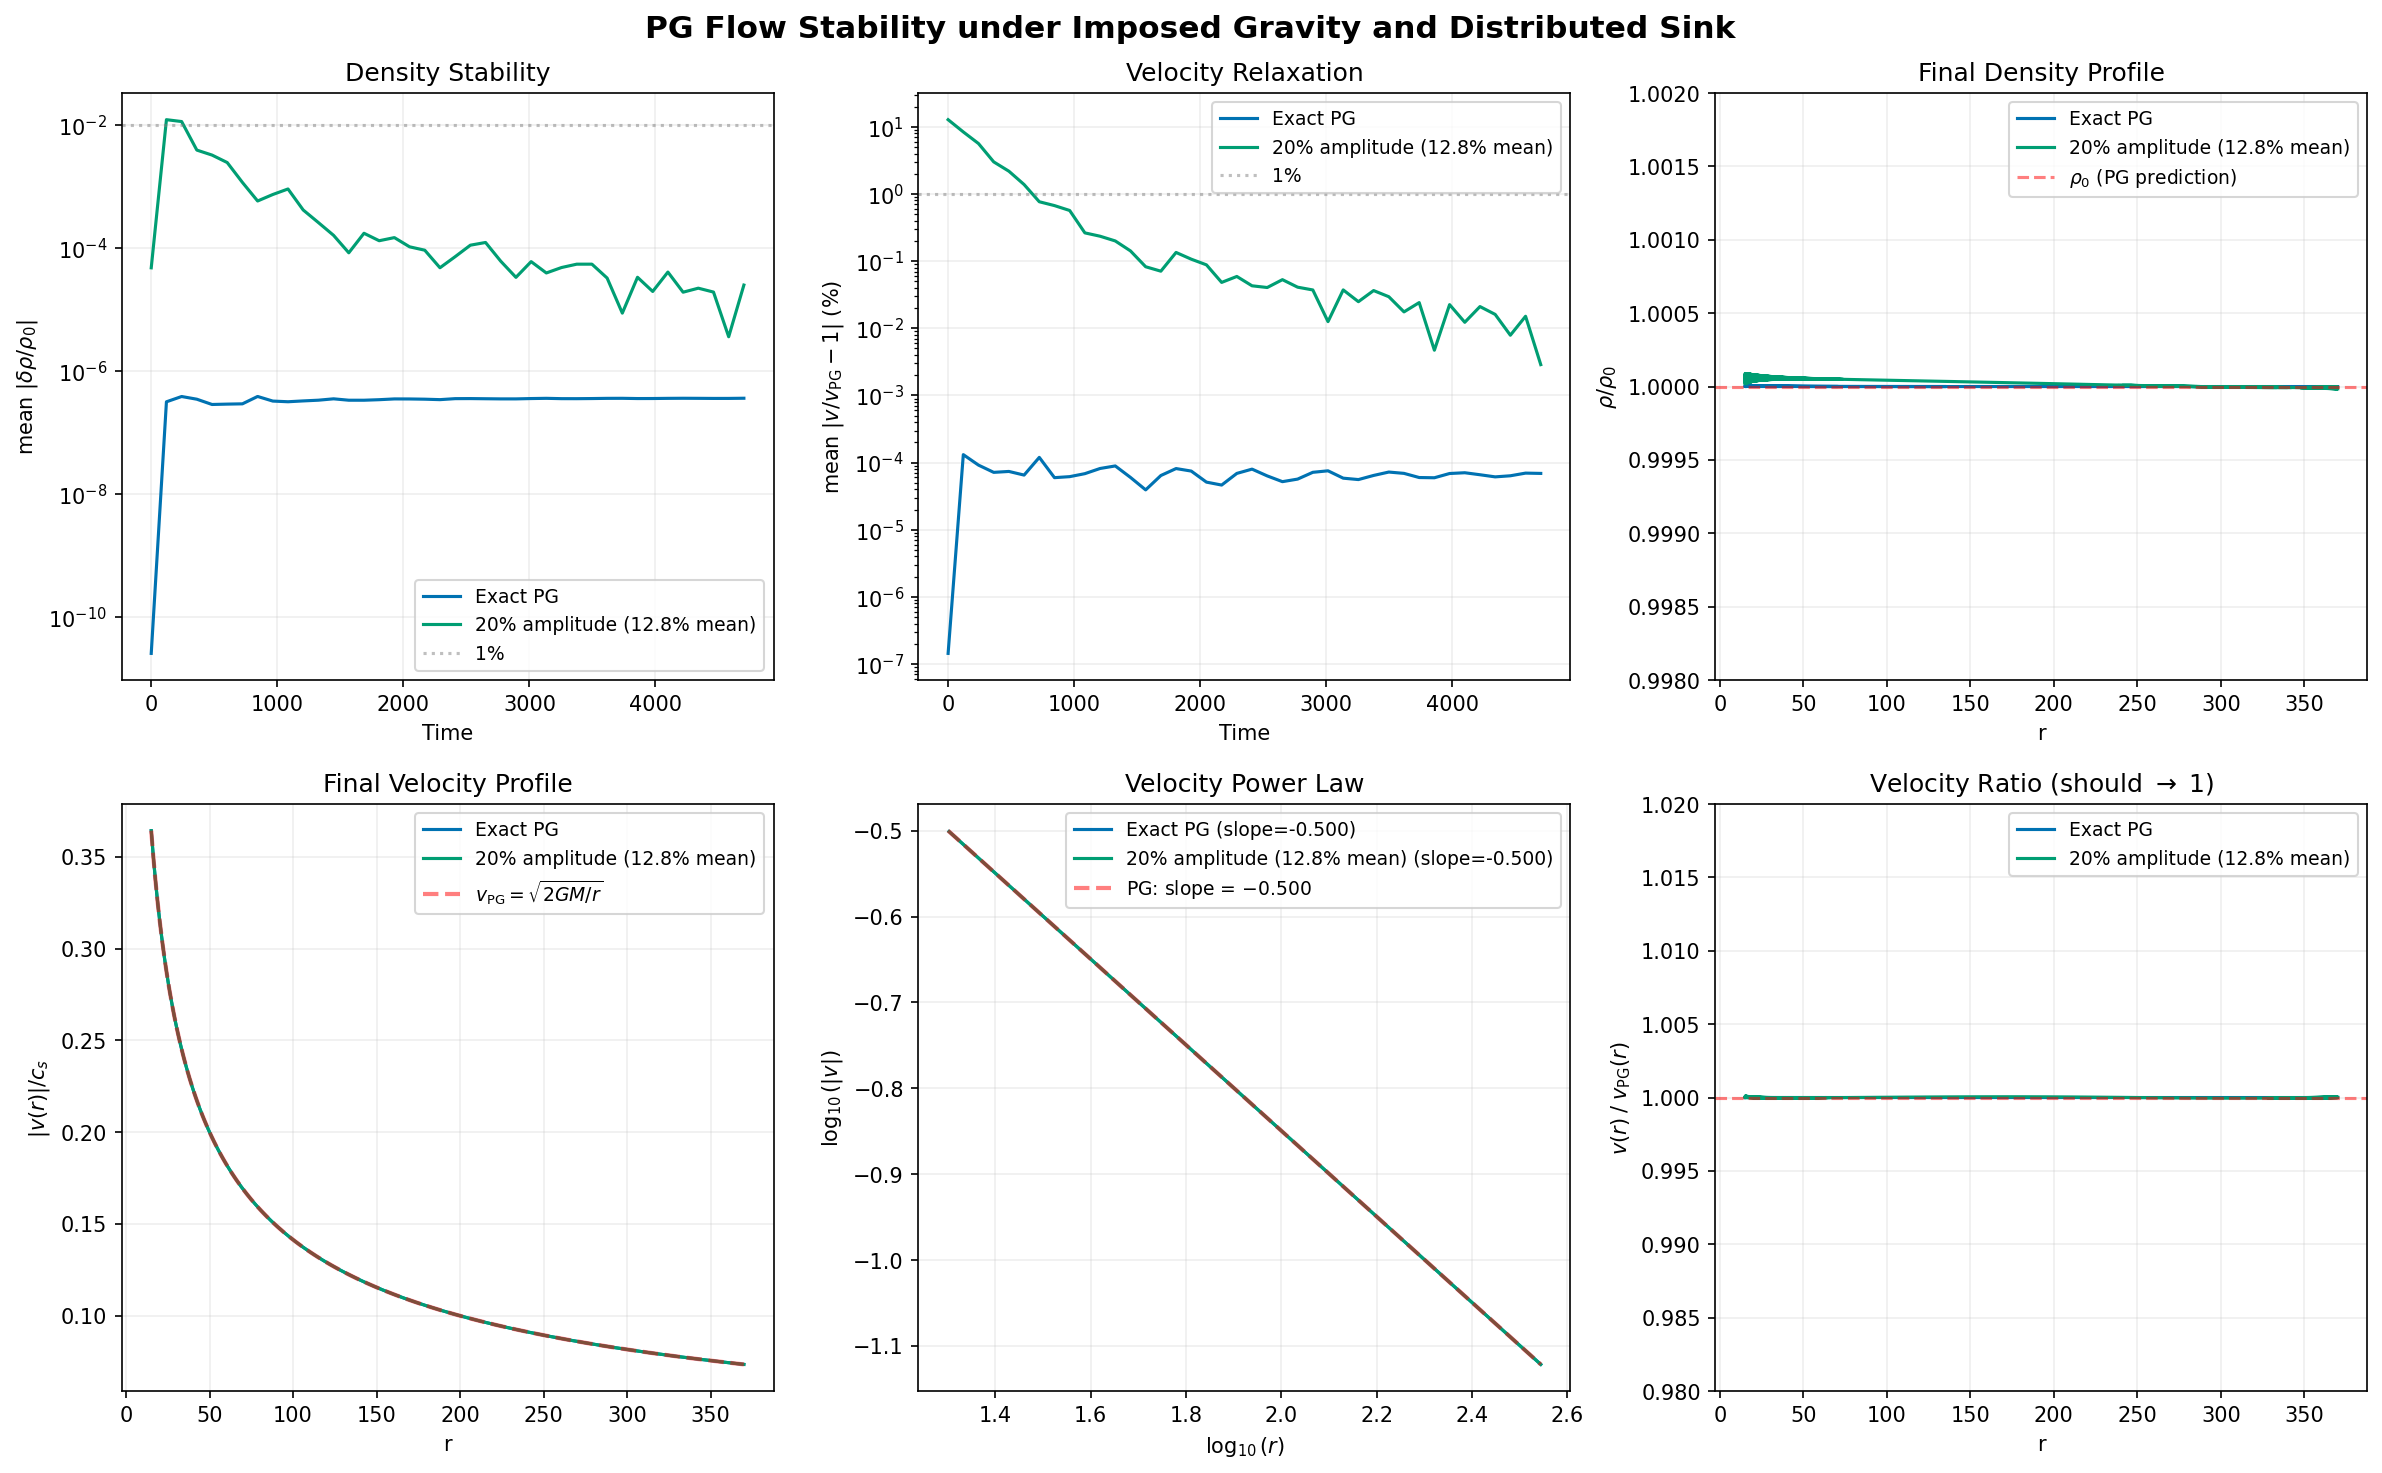
\includegraphics[width=\textwidth]{pg_distributed_sink.png}
\caption{\emph{Top row, left to right:} density deviation and velocity error versus time for exact PG (blue) and 20\% velocity perturbation (green); final density profile.
\emph{Bottom row:} final velocity profile compared with $v_{\mathrm{PG}} = \sqrt{2GM/r}$ (dashed red); velocity power law with measured slopes; velocity ratio $v/v_{\mathrm{PG}}$. Both cases converge to $v \propto r^{-0.500}$ with $\rho/\rho_0 = 1$ to within $10^{-4}$.}
\label{fig:pg_numerical}
\end{figure}

% ====================================================================
\section{Discussion}
\label{sec:discussion}
% ====================================================================

\subsection{The logical chain}

Our results establish a complete chain from microscopic to macroscopic:

\paragraph{Building block} Each particle is a vortex-Gausson soliton of size $\sim\xi$, energy $E_v$, and mass $m$, with topologically locked circulation $v_\theta \propto 1/r$ (Sec.~\ref{sec:numerics}).

\paragraph{Collective source} $N = M/m$ solitons create a coarse-grained source $T_{00}(r) = n(r)\cdot E_v$ in the condensate (Sec.~\ref{sec:framework}).

\paragraph{Acoustic metric response} The linearized acoustic perturbation equations give a Newtonian potential $\Phieff = -\Geff M/r$ with $\Geff \sim c^2/(\xi^2\rho_0)$ (Sec.~\ref{sec:G_eff}).

\paragraph{Self-consistency selects PG} The PG flow $\vb = \sqrt{2\Geff M/r}$ is the unique weak-field solution whose acoustic metric reproduces the assumed gravitational potential. The static solution fails this test (Sec.~\ref{sec:self_consistency}).

\paragraph{Bernoulli confirms} The Bernoulli relation $\delta\rho \propto v^2$, combined with Newtonian $\delta\rho \propto 1/r$, independently requires $v \propto 1/\sqrt{r}$ (Sec.~\ref{sec:bernoulli}).


\subsection{The continuity constraint}
\label{sec:continuity}

The PG flow has nonzero divergence:
\begin{equation}
    \nabla\cdot\vb = \frac{3}{2}\sqrt{\frac{2\Geff M}{r^3}} \neq 0\,.
\end{equation}
In a strictly steady state with $\rhob \approx \rho_0$, this violates the continuity equation~(\ref{eq:cg_continuity}) unless balanced by a source or sink.

Several mechanisms could provide this balance:

\paragraph{Quasi-steady approximation} The density buildup rate $\partial\rho/\partial t = -\rho_0\,\nabla\cdot\vb$ produces fractional changes $\delta\rho/\rho_0 \sim U \sim 10^{-6}$ per free-fall time ($\sim 30$~min at the solar limb). Over any practical observation timescale, this is negligible, and the PG flow is an excellent quasi-steady approximation.

\paragraph{Two-fluid counterflow} In superfluid helium, heat transport occurs via counterflow: the superfluid component flows one direction while the normal (thermal) component flows the opposite way, maintaining zero net mass current~\cite{volovik_2003}. Applied here, the superfluid inflow creating the PG metric could be balanced by an outward normal-component flow, giving $\nabla\cdot(\rho_s \mathbf{v}_s + \rho_n\mathbf{v}_n) = 0$ even though $\nabla\cdot\mathbf{v}_s \neq 0$.

\paragraph{Vortex-core absorption} Each soliton core ($\rho \to 0$ at $r = 0$) acts as a sink for the background condensate. The absorption rate $\Gamma_{\mathrm{sink}}$ per particle, summed over $N$ particles, could balance the PG inflow. This requires $N\,\Gamma_{\mathrm{sink}} = 4\pi r^2 \rho_0\,v(r)$ for all $r$, which is only satisfied at the sonic point; outside this radius, the quasi-steady approximation applies.

\paragraph{Geometric redirection} The radial PG inflow may be continuously redirected into non-radial outflow---for example, into a collimated polar jet along the rotation axis of the gravitating body. Continuity is then satisfied globally: condensate flowing in radially flows out axially, with no local accumulation. The mathematical analysis of this mechanism is the subject of separate work.

The choice of mechanism is deferred to future work. All four are consistent with the weak-field PG solution analyzed here; distinguishing between them requires analysis of the strong-field regime near compact objects or of the steady-state structure of the condensate at galactic and cosmological scales.


\subsection{The vacuum density and the cosmological constant problem}

The predicted vacuum mass density $\rho_0 \sim m_P/\lP^3 \approx 5 \times 10^{96}$~kg/m$^3$ (Eq.~\ref{eq:planck_scale}) is the natural Planck-scale density for a relativistic quantum field. The corresponding bulk modulus $K = \rho_0 c^2 \sim 10^{113}$~Pa quantifies the vacuum's stiffness: gravity is weak because the substrate resists deformation enormously, requiring macroscopic source masses to produce measurable perturbations of the condensate.

The energy density of the background condensate, $\rho_0 c^2 \sim 10^{113}$~J/m$^3$, is comparable to the QFT zero-point estimate of the cosmological constant. In the present framework, however, this background energy is \emph{not} directly observable: gravitational effects are sourced by perturbations $\delta\rho/\rho_0 \sim U$ around the background, not by the background density itself. The observed dark energy density ($\sim 10^{-9}$~J/m$^3$) is therefore not in conflict with $\rho_0 c^2 \sim 10^{113}$~J/m$^3$; the question shifts from ``why is the vacuum energy so small'' to ``why is the relevant cosmological perturbation so small,'' a distinction that deserves separate investigation.

\subsection{Thermodynamic stability of the vacuum density}

The requirement that $\rho_0$ remain approximately constant across cosmic time is supported by a thermodynamic feature of the logarithmic potential. For $V(\rho) = -b\,\rho\,\ln(\rho/\rho_c)$, the macroscopic pressure at the background density is:
\begin{equation}
    P = \rho\,\frac{\partial V}{\partial\rho} - V = -b\,\rho_0\,.
\label{eq:pressure}
\end{equation}
With $b$ normalized so that $c_s = c$ at the background density, this gives $P \approx -\rho_0 c^2$, i.e.\ an equation of state parameter $w = P/(\rho_0 c^2) = -1$. Through the first law of thermodynamics, the expansion of cosmic volume performs work against this tension, and the cosmological density parameter scales as $\rho \propto a^{-3(1+w)} = a^0 = \text{const}$. The mechanism by which this is realized---whether through open-system condensate accretion, intrinsic potential-minimum stability, or another mechanism---is beyond the scope of the present analysis and is developed elsewhere.

\subsection{Predictions and tests}

The framework makes several testable predictions:

\paragraph{Gravitational light bending} $\gamma = 1$ exactly, matching GR and the Cassini measurement~\cite{bertotti_2003}. This is a postdiction, not a prediction, but it is a necessary consistency check that the model passes.

\paragraph{Speed of gravity} The acoustic metric~(\ref{eq:acoustic_metric}) predicts that gravitational perturbations propagate at $c_s = c$, consistent with the GW170817 constraint~\cite{abbott_2017}.

\paragraph{No gravitational reflection} In the PG flow solution with $\rhob \approx \rho_0$, there is no significant impedance mismatch at macroscopic scales: the density is nearly uniform and the sound speed is nearly constant. The model does not predict observable gravitational echoes at solar system scales.

\paragraph{Vacuum density} The prediction $\rho_0 \sim m_P/\lP^3 \sim 10^{96}$~kg/m$^3$ (Planck density) could in principle be constrained by high-precision measurements of $G$ and $c$ across cosmic time: any drift of $\rho_0$ or $\xi$ would produce a time-dependent $G$. Current bounds on $\dot G/G < 10^{-13}$~yr$^{-1}$~\cite{will_2014} are consistent with a static condensate.


% ====================================================================
\section{Conclusion}
\label{sec:conclusion}
% ====================================================================

We have derived the macroscopic PG flow as a collective
mean-field effect of microscopic vortex-Gausson solitons in the logarithmic condensate, completing the emergent gravity program initiated in~\cite{kulangiev_2026}. The key results are:

(1) The self-consistency of the acoustic metric equations uniquely selects the Painlev\'{e}-Gullstrand flow $v = \sqrt{2\Geff M/r}$, yielding $\gamma = 1$ for any barotropic equation of state. The static solution is inconsistent.

(2) The Bernoulli relation of the logarithmic fluid
independently confirms that Newtonian gravity requires
$v^2 \propto 1/r$.

(3) The emergent gravitational constant $\Geff \sim c^2/(\xi^2\rho_0)$ is universal. Combined with the soliton healing-length structure and the natural condensate packing density, self-consistency fixes $\xi \sim \lP$ and $\rho_0 \sim m_P/\lP^3$ (Planck scale).

(4) The first-order density depletion from the PG flow, $\epsilon = -U$, decouples from the temporal metric at the background exponent $\alpha = -1$, so the vacuum around a gravitating mass is gravitationally indistinguishable from free vacuum at the $10^{-12}$ level even though its density is perturbed at $O(U)$.

The apparent continuity constraint of the macroscopic PG inflow remains an open problem. Among the candidate mechanisms discussed in Sec.~\ref{sec:continuity}, the geometric-redirection option---where rotation defines a polar axis and the radial inflow is balanced by axial outflow at large angles from the equatorial plane---is mathematically attractive but requires a proper axisymmetric analysis beyond the present scope. The formal derivation of the macroscopic PG flow as a collective Bernoulli response of $N$ microscopic vortex-Gaussons to the mean-field gravitational potential---the gravitational analogue of the Feynman-Onsager relation in rotating superfluids---is left to future work.


% ====================================================================
\section*{Acknowledgments}

The author thanks C.~Barcel\'{o}, S.~Liberati, and M.~Visser for the acoustic metric framework. The methodological stance of this paper---treating the order parameter as a real classical field whose hydrodynamic behavior underlies emergent gravitational phenomena---is indebted to the Madelung-de~Broglie-Bohm tradition, particularly as developed in P.~R.~Holland's exposition of the quantum theory of motion. Claude (Anthropic) and Gemini (Google) were used as editorial and computational tools during manuscript preparation. All scientific content, equations, and interpretations are the author's own.


\begin{thebibliography}{25}

\bibitem{kulangiev_2026}
B.~B.~Kulangiev,
Conditions for Emergent Gravitational Light Bending from a Logarithmic Superfluid Vacuum,
Preprint (2026).
\url{https://kulangiev.github.io#paper1}

\bibitem{kulangiev_2026e}
B.~B.~Kulangiev,
Singularity Regularization and the Emergent Planck Scale in the Logarithmic Superfluid Vacuum,
Preprint (2026).
\url{https://kulangiev.github.io#paper5}

\bibitem{rosen_1969}
G.~Rosen,
``Dilatation covariance and exact solutions in local relativistic field theories,''
Phys.\ Rev.\ \textbf{183}, 1186 (1969).

\bibitem{bialynicki_birula_1979}
I.~Bia\l{}ynicki-Birula and J.~Mycielski,
Gaussons: Solitons of the logarithmic Schr\"{o}dinger equation,
Phys.\ Scr.\ \textbf{20}, 539 (1979).

\bibitem{bartkowski_gorka_2008}
K.~Bartkowski and P.~G\'{o}rka,
``One-dimensional Klein-Gordon equation with logarithmic nonlinearities,''
J.\ Phys.\ A: Math.\ Theor.\ \textbf{41}, 355201 (2008).

\bibitem{avdeenkov_2011}
A.~V.~Avdeenkov and K.~G.~Zloshchastiev,
Quantum Bose liquids with logarithmic nonlinearity: Self-sustainability and emergence of spatial extent,
J.\ Phys.\ B \textbf{44}, 195303 (2011).

\bibitem{unruh_1981}
W.~G.~Unruh,
Experimental black-hole evaporation?,
Phys.\ Rev.\ Lett.\ \textbf{46}, 1351 (1981).

\bibitem{visser_1998}
M.~Visser,
Acoustic black holes: Horizons, ergospheres and Hawking radiation,
Class.\ Quant.\ Grav.\ \textbf{15}, 1767 (1998).

\bibitem{volovik_2003}
G.~E.~Volovik,
\emph{The Universe in a Helium Droplet} (Oxford, 2003).

\bibitem{bertotti_2003}
B.~Bertotti, L.~Iess, and P.~Tortora,
A test of general relativity using radio links with the Cassini spacecraft,
Nature \textbf{425}, 374 (2003).

\bibitem{abbott_2017}
B.~P.~Abbott \emph{et al.},
Gravitational waves and gamma-rays from a binary neutron star merger: GW170817 and GRB~170817A,
Astrophys.\ J.\ Lett.\ \textbf{848}, L13 (2017).

\bibitem{will_2014}
C.~M.~Will,
\emph{Theory and Experiment in Gravitational Physics}, 2nd ed.\ (Cambridge, 2014).

\bibitem{barcelo_2005}
C.~Barcel\'{o}, S.~Liberati, and M.~Visser,
Analogue gravity,
Living Rev.\ Rel.\ \textbf{8}, 12 (2005);
updated: \textbf{14}, 3 (2011).

\end{thebibliography}

\end{document}
